% Chapter 14: Fractal Market Hypothesis
% Harvard-quality academic presentation
% Bachelor program, Bucharest University of Economic Studies

\documentclass[9pt, aspectratio=169, t]{beamer}

% Ensure content fits on slides
\setbeamersize{text margin left=8mm, text margin right=8mm}

%=============================================================================
% THEME AND STYLE CONFIGURATION
%=============================================================================
\usetheme{default}
% Using default theme for clean header/footer control

% Color Palette (matching Redispatch PDF)
\definecolor{MainBlue}{RGB}{26, 58, 110}
\definecolor{AccentBlue}{RGB}{26, 58, 110}
\definecolor{IDAred}{RGB}{205, 0, 0}
\definecolor{DarkGray}{RGB}{51, 51, 51}
\definecolor{MediumGray}{RGB}{128, 128, 128}
\definecolor{LightGray}{RGB}{248, 248, 248}
\definecolor{VeryLightGray}{RGB}{235, 235, 235}
\definecolor{KeynoteGray}{RGB}{218, 218, 218}
\definecolor{SectionGray}{RGB}{120, 120, 120}
\definecolor{FooterGray}{RGB}{100, 100, 100}
\definecolor{Crimson}{RGB}{220, 53, 69}
\definecolor{Forest}{RGB}{46, 125, 50}
\definecolor{Amber}{RGB}{181, 133, 63}
\definecolor{Orange}{RGB}{230, 126, 34}
\definecolor{Purple}{RGB}{142, 68, 173}

% Gradient background (exact Keynote 315° gradient: white to RGB 218,218,218)
\setbeamertemplate{background}{%
    \begin{tikzpicture}[remember picture, overlay]
        \shade[shading=axis, shading angle=315,
        top color=white, bottom color=KeynoteGray]
        (current page.south west) rectangle (current page.north east);
    \end{tikzpicture}%
}
% Fallback solid color for compatibility
\setbeamercolor{background canvas}{bg=}

\setbeamercolor{palette primary}{bg=MainBlue, fg=white}
\setbeamercolor{palette secondary}{bg=MainBlue!85, fg=white}
\setbeamercolor{palette tertiary}{bg=MainBlue!70, fg=white}
\setbeamercolor{structure}{fg=MainBlue}
\setbeamercolor{title}{fg=IDAred}
\setbeamercolor{frametitle}{fg=IDAred, bg=}
\setbeamercolor{block title}{bg=MainBlue, fg=white}
\setbeamercolor{block body}{bg=VeryLightGray, fg=DarkGray}
\setbeamercolor{block title alerted}{bg=Crimson, fg=white}
\setbeamercolor{block body alerted}{bg=Crimson!8, fg=DarkGray}
\setbeamercolor{block title example}{bg=Forest, fg=white}
\setbeamercolor{block body example}{bg=Forest!8, fg=DarkGray}
\setbeamercolor{item}{fg=MainBlue}

% Footer colors (override Madrid theme blue)
\setbeamercolor{author in head/foot}{fg=FooterGray, bg=}
\setbeamercolor{title in head/foot}{fg=FooterGray, bg=}
\setbeamercolor{date in head/foot}{fg=FooterGray, bg=}
\setbeamercolor{section in head/foot}{fg=FooterGray, bg=}
\setbeamercolor{subsection in head/foot}{fg=FooterGray, bg=}

% Bullet styles (apply everywhere including blocks)
\setbeamertemplate{itemize item}{\color{MainBlue}$\boxdot$}
\setbeamertemplate{itemize subitem}{\color{MainBlue}$\blacktriangleright$}
\setbeamertemplate{itemize subsubitem}{\color{MainBlue}\tiny$\bullet$}
\setbeamertemplate{itemize/enumerate body begin}{\normalsize}
\setbeamertemplate{itemize/enumerate subbody begin}{\normalsize}

% Item spacing - compact style
\setlength{\leftmargini}{10pt}       % Level 1: minimal indent
\setlength{\leftmarginii}{10pt}      % Level 2: minimal additional indent
% Compact list spacing (zero extra space before/after lists in blocks)
\makeatletter
\def\@listi{\leftmargin\leftmargini \topsep 0pt \parsep 0pt \itemsep 0pt}
\def\@listii{\leftmargin\leftmarginii \topsep 0pt \parsep 0pt \itemsep 0pt}
\makeatother

\setbeamertemplate{navigation symbols}{}

%=============================================================================
% CUSTOM HEADLINE
%=============================================================================
\setbeamertemplate{headline}{%
    \vskip10pt%
    \hbox to \paperwidth{%
        \hskip0.5cm%
        {\small\color{FooterGray}\renewcommand{\hyperlink}[2]{##2}\insertsectionhead}%
        \hfill%
        \textcolor{FooterGray}{\small\insertframenumber}%
        \hskip0.5cm%
    }%
    \vskip4pt%
    {\color{FooterGray}\hrule height 0.4pt}%
}

%=============================================================================
% CUSTOM FOOTER
%=============================================================================
\usepackage{fontawesome5}

\setbeamertemplate{footline}{%
    {\color{FooterGray}\hrule height 0.4pt}%
    \vskip4pt%
    \hbox to \paperwidth{%
        \hskip0.5cm%
        \textcolor{FooterGray}{\small Statistics of Financial Markets}%
        \hfill%
        \raisebox{-0.1em}{%
            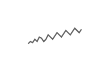
\begin{tikzpicture}[x=0.08em, y=0.08em, line width=0.4pt]
                \draw[FooterGray] (0,3) -- (1,4) -- (2,3.5) -- (3,5) -- (4,4) -- (5,6) -- (6,5.5) -- (7,4) -- (8,5) -- (9,7) -- (10,6) -- (11,5) -- (12,6.5) -- (13,8) -- (14,7) -- (15,6) -- (16,7.5) -- (17,9) -- (18,8) -- (19,7) -- (20,8.5) -- (21,10) -- (22,9) -- (23,8) -- (24,9.5);
            \end{tikzpicture}%
        }%
        \hskip0.5cm%
    }%
    \vskip6pt%
}

%=============================================================================
% PACKAGES
%=============================================================================
\usepackage[utf8]{inputenc}
\usepackage[T1]{fontenc}
\usepackage{amsmath, amssymb, amsthm}
\usepackage{mathtools}
\usepackage{bm}
\usepackage{tikz}
\usetikzlibrary{arrows.meta, positioning, shapes, calc, decorations.pathreplacing, shadings}
\usepackage{booktabs}
\usepackage{multirow}
\usepackage{array}
\usepackage{graphicx}
\usepackage{hyperref}
\usepackage{colortbl}
\usepackage{listings}
\lstset{language=Python, basicstyle=\ttfamily\scriptsize, keywordstyle=\color{MainBlue}\bfseries,
  commentstyle=\color{Forest}, stringstyle=\color{Crimson}, breaklines=true,
  frame=none, backgroundcolor=\color{VeryLightGray}, xleftmargin=2mm}
\hypersetup{colorlinks=true, linkcolor=MainBlue, urlcolor=MainBlue}
\graphicspath{{../../logos/}{../../charts/}{../../photos/}}
\hfuzz=2pt  % Suppress tiny overfull warnings (<2pt)
\vfuzz=2pt  % Suppress tiny vertical overfull warnings (<2pt)

%=============================================================================
% QUANTLET COMMAND
%=============================================================================
\newcommand{\quantlet}[2]{%
    \hfill\href{#2}{%
        \raisebox{-0.15em}{
\includegraphics[height=0.7em]{ql_logo.png}}%
        \textcolor{MainBlue}{\tiny\ #1}%
    }%
}

%=============================================================================
% CUSTOM TITLE PAGE
%=============================================================================
\defbeamertemplate*{title page}{hybrid}[1][]
{
    \vspace{0.2cm}
    % Logos row - top header (with clickable links)
    \begin{center}
        \href{https://www.ase.ro}{
\includegraphics[height=1.0cm]{ase_logo.png}}\hspace{0.3cm}%
        \href{https://theida.net}{
\includegraphics[height=1.0cm]{ida_logo.png}}\hspace{0.3cm}%
        \href{https://blockchain-research-center.com}{
\includegraphics[height=1.0cm]{brc_logo.png}}\hspace{0.3cm}%
        \href{https://www.ai4efin.ase.ro}{
\includegraphics[height=1.0cm]{ai4efin_logo.png}}\hspace{0.3cm}%
        \href{https://ipe.ro/new}{
\includegraphics[height=1.0cm]{acad_logo.png}}\hspace{0.3cm}%
        \href{https://www.digital-finance-msca.com}{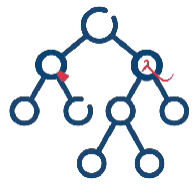
\includegraphics[height=1.0cm]{msca_logo.png}}%
    \end{center}

    \vspace{0.6cm}

    % Main title with Q logos on sides (with clickable links)
    \begin{center}
        \begin{minipage}{0.1\textwidth}
            \centering
            \href{https://quantlet.com}{
\includegraphics[height=1.1cm]{ql_logo.png}}
        \end{minipage}%
        \begin{minipage}{0.78\textwidth}
            \centering
            {\LARGE\bfseries\usebeamercolor[fg]{title}\inserttitle}

            \vspace{0.3cm}

            {\usebeamerfont{subtitle}\usebeamercolor[fg]{title}\insertsubtitle}
        \end{minipage}%
        \begin{minipage}{0.1\textwidth}
            \centering
            \href{https://quantinar.com}{
\includegraphics[height=1.1cm]{qr_logo.png}}
        \end{minipage}
    \end{center}

    \vspace{0.6cm}

    % Authors (left aligned)
    \hspace{0.5cm}{\usebeamerfont{author}\insertauthor}

    \vspace{0.3cm}

    % Institute/Affiliations (left aligned)
    \hspace{0.5cm}\begin{minipage}[t]{0.9\textwidth}
        \raggedright\small\insertinstitute
    \end{minipage}
}

%=============================================================================
% THEOREM ENVIRONMENTS
%=============================================================================
\theoremstyle{definition}
\setbeamertemplate{theorems}[numbered]
\newtheorem{defn}{Definition}
\newtheorem{thm}{Theorem}
\newtheorem{prop}{Proposition}
\newtheorem{rmk}{Remark}

%=============================================================================
% CENTRED MINIPAGE (no extra vertical space)
%=============================================================================
\newenvironment{cminipage}[1]{%
    \par\noindent\hfill\begin{minipage}{#1}\ignorespaces
}{%
    \end{minipage}\hfill\null\par
}

%=============================================================================
% CUSTOM COMMANDS
%=============================================================================
\newcommand{\E}{\mathbb{E}}
\newcommand{\Var}{\text{Var}}
\newcommand{\Cov}{\text{Cov}}
\newcommand{\Corr}{\text{Corr}}
\newcommand{\R}{\mathbb{R}}
\newcommand{\N}{\mathbb{N}}
\newcommand{\Z}{\mathbb{Z}}
\newcommand{\B}{\mathbf{B}}
\newcommand{\imark}{\textcolor{MainBlue}{\textbullet}}
\newcommand{\RMSE}{\text{RMSE}}
\newcommand{\MAE}{\text{MAE}}
\newcommand{\MAPE}{\text{MAPE}}

%=============================================================================
% TITLE INFORMATION
%=============================================================================
\title[Statistics of Financial Markets]{Statistics of Financial Markets}
\subtitle{Chapter 14: Fractal Market Hypothesis}
\author[D.T. Pele, S. Gaman]{Daniel Traian PELE \\ Stefan Gaman}
\institute{Bucharest University of Economic Studies\\
IDA Institute Digital Assets\\
Blockchain Research Center\\
AI4EFin Artificial Intelligence for Energy Finance\\
Romanian Academy, Institute for Economic Forecasting\\
MSCA Digital Finance}
\date{}

%=============================================================================
\begin{document}
%=============================================================================

% Title page
{
\setbeamertemplate{headline}{}
\setbeamertemplate{footline}{}
\begin{frame}[noframenumbering]
    \titlepage
\end{frame}
}

%=============================================================================
% OUTLINE
%=============================================================================
\begin{frame}{Outline}
    \tableofcontents
\end{frame}

%=============================================================================
% SECTION 1: Motivation
%=============================================================================
\section{Motivation}

\begin{frame}{Motivation}
    \begin{itemize}
        \item The \textbf{Efficient Market Hypothesis} (EMH) of Fama (1970) has been the dominant paradigm in financial economics for over half a century
        \item EMH assumes that asset prices fully reflect all available information and that returns follow a random walk with i.i.d.\ Gaussian innovations:
        \[
            r_t = \mu + \varepsilon_t, \qquad \varepsilon_t \overset{\text{i.i.d.}}{\sim} \mathcal{N}(0, \sigma^2)
        \]
        \item However, EMH \textbf{fails to explain} several empirical regularities:
        \begin{itemize}
            \item \textbf{Fat tails}: $\Pr(|r_t| > x) \gg \Phi(-x)$ for large $x$, i.e.\ return distributions exhibit excess kurtosis $\kappa > 3$
            \item \textbf{Volatility clustering}: large returns tend to follow large returns, $\Corr(|r_t|, |r_{t+k}|) > 0$ for many lags $k$
            \item \textbf{Long memory}: slow decay of autocorrelations, $\rho(k) \sim C k^{2H-2}$ as $k \to \infty$ for $H > 0.5$
            \item \textbf{Market crashes}: sudden, correlated drops that are orders of magnitude beyond Gaussian predictions (e.g., Black Monday 1987: $-22.6\%$)
        \end{itemize}
        \item The \textbf{Fractal Market Hypothesis} (FMH), proposed by Peters (1991, 1994), offers an alternative framework based on fractal geometry, heterogeneous time horizons, and the concept of market liquidity
    \end{itemize}
\end{frame}

\begin{frame}{EMH vs FMH}
    \begin{columns}[T]
        \begin{column}{0.48\textwidth}
            \begin{block}{Efficient Market Hypothesis (EMH)}
                \begin{itemize}
                    \item All investors have \textbf{the same investment horizon} and react identically to information
                    \item Information is \textbf{immediately and fully} reflected in asset prices
                    \item Returns are \textbf{i.i.d.} with a well-defined variance:
                    \[
                        r_t \overset{\text{i.i.d.}}{\sim} F(\mu, \sigma^2)
                    \]
                    \item Markets are always in \textbf{equilibrium}; arbitrage opportunities vanish instantaneously
                    \item Price changes follow a \textbf{random walk} $\succ$ no serial dependence
                    \item Risk is fully captured by \textbf{variance} $\sigma^2$ (mean-variance framework)
                \end{itemize}
            \end{block}
        \end{column}
        \begin{column}{0.48\textwidth}
            \begin{block}{Fractal Market Hypothesis (FMH)}
                \begin{itemize}
                    \item Investors operate on \textbf{multiple time horizons}: from intraday to multi-year
                    \item Information is \textbf{valued differently} depending on the investor's horizon
                    \item Market \textbf{stability} depends on the \textbf{diversity of horizons}:
                    \[
                        \text{Liquidity} \propto \text{Horizon diversity}
                    \]
                    \item When horizons \textbf{collapse} (all investors panic simultaneously), liquidity evaporates and crashes occur
                    \item Returns exhibit \textbf{self-similarity} and \textbf{long-range dependence}
                    \item Risk is characterized by the \textbf{Hurst exponent} $H$ and the full distributional shape
                \end{itemize}
            \end{block}
        \end{column}
    \end{columns}
\end{frame}

%=============================================================================
% SECTION 2: Fractals in Finance
%=============================================================================
\section{Fractals in Finance}

\begin{frame}{Self-Similarity}
    \begin{defn}[Statistical Self-Similarity]
        A stochastic process $\{X(t)\}_{t \geq 0}$ is called \textbf{self-similar} with index $H > 0$ (or $H$-ss) if for every $c > 0$:
        \[
            \{X(ct)\}_{t \geq 0} \stackrel{d}{=} \{c^H X(t)\}_{t \geq 0}
        \]
        where $\stackrel{d}{=}$ denotes equality of all finite-dimensional distributions.
    \end{defn}
    \begin{itemize}
        \item The parameter $H$ is called the \textbf{self-similarity exponent} (or Hurst exponent)
        \item \textbf{Implications for returns}: if the log-price process $\ln P(t)$ is $H$-self-similar, then rescaling time by $c$ is equivalent to rescaling returns by $c^H$:
        \[
            r(t, \Delta) = \ln P(t+\Delta) - \ln P(t) \stackrel{d}{=} c^H \, r\!\left(\frac{t}{c}, \frac{\Delta}{c}\right)
        \]
        \item For returns over horizon $\Delta$, the \textbf{volatility scaling law} follows:
        \[
            \sigma(\Delta) = \sigma(1) \cdot \Delta^{H}
        \]
        \item Under EMH ($H = 0.5$), this gives the classical square-root-of-time rule: $\sigma(\Delta) = \sigma(1) \sqrt{\Delta}$
        \item For $H \neq 0.5$, the scaling deviates $\succ$ evidence \textbf{against} EMH
    \end{itemize}
\end{frame}

\begin{frame}{Fractional Brownian Motion}
    \begin{defn}[Fractional Brownian Motion]
        A \textbf{fractional Brownian motion} (fBm) $\{B_H(t)\}_{t \in \R}$ with Hurst parameter $H \in (0,1)$ is the unique centered Gaussian process with $B_H(0) = 0$ and covariance:
        \[
            \E[B_H(t) \, B_H(s)] = \frac{1}{2}\bigl(|t|^{2H} + |s|^{2H} - |t-s|^{2H}\bigr)
        \]
    \end{defn}
    \begin{itemize}
        \item \textbf{Key properties} of fBm:
        \begin{itemize}
            \item Self-similar with exponent $H$: $B_H(ct) \stackrel{d}{=} c^H B_H(t)$
            \item Stationary increments: $B_H(t+s) - B_H(s) \stackrel{d}{=} B_H(t)$
            \item Variance of increments: $\E[(B_H(t) - B_H(s))^2] = |t-s|^{2H}$
        \end{itemize}
        \item \textbf{Three regimes} based on $H$:
        \begin{itemize}
            \item $H = 0.5$: \textbf{Standard Brownian motion} $\succ$ independent increments, no memory
            \item $H > 0.5$: \textbf{Persistent} (trending) $\succ$ positive autocorrelation of increments, $\Corr(\Delta B_H(t), \Delta B_H(t+k)) > 0$
            \item $H < 0.5$: \textbf{Anti-persistent} (mean-reverting) $\succ$ negative autocorrelation, $\Corr(\Delta B_H(t), \Delta B_H(t+k)) < 0$
        \end{itemize}
        \item The autocovariance of increments at lag $k$ is:
        \[
            \gamma(k) = \frac{1}{2}\bigl(|k+1|^{2H} - 2|k|^{2H} + |k-1|^{2H}\bigr) \approx H(2H-1)|k|^{2H-2} \text{ as } k \to \infty
        \]
    \end{itemize}
\end{frame}

\begin{frame}{Long Memory Processes}
    \begin{defn}[ARFIMA Process]
        A process $\{y_t\}$ follows an \textbf{ARFIMA}$(p,d,q)$ model if:
        \[
            \Phi(L)(1-L)^d y_t = \Theta(L)\varepsilon_t, \qquad \varepsilon_t \overset{\text{i.i.d.}}{\sim} (0, \sigma^2_\varepsilon)
        \]
        where $d \in (-0.5, 0.5)$ is the fractional differencing parameter, $\Phi(L) = 1 - \phi_1 L - \cdots - \phi_p L^p$ is the AR polynomial, and $\Theta(L) = 1 + \theta_1 L + \cdots + \theta_q L^q$ is the MA polynomial.
    \end{defn}
    \begin{itemize}
        \item The \textbf{fractional difference operator} $(1-L)^d$ is defined via its binomial expansion:
        \[
            (1-L)^d = \sum_{k=0}^{\infty} \binom{d}{k} (-L)^k = 1 - dL - \frac{d(1-d)}{2!}L^2 - \frac{d(1-d)(2-d)}{3!}L^3 - \cdots
        \]
        \item \textbf{Connection to the Hurst exponent}: for a pure ARFIMA$(0,d,0)$ process,
        \[
            d = H - \frac{1}{2}
        \]
        \item The spectral density near frequency zero behaves as $f(\lambda) \sim C_f |\lambda|^{-2d}$ as $\lambda \to 0$
        \item \textbf{Long memory} ($0 < d < 0.5$, equivalently $H > 0.5$): the autocorrelation function decays hyperbolically, $\rho(k) \sim C \, k^{2d-1}$ as $k \to \infty$, and $\sum_{k=-\infty}^{\infty} |\rho(k)| = \infty$
        \item \textbf{Short memory} ($d = 0$, equivalently $H = 0.5$): autocorrelations decay exponentially, typical of standard ARMA processes
    \end{itemize}
\end{frame}

%=============================================================================
% SECTION 3: The Hurst Exponent
%=============================================================================
\section{The Hurst Exponent}

\begin{frame}{Hurst Exponent: Definition}
    \begin{itemize}
        \item Named after \textbf{Harold Edwin Hurst} (1880--1978), a British hydrologist who studied the long-term storage capacity of the Nile River
        \item Hurst (1951) found that the annual minima and maxima of the Nile's water levels exhibited \textbf{long-range dependence}: wet years tended to cluster, as did dry years
        \item He discovered that the rescaled range $R/S$ scaled as $n^H$ with $H \approx 0.73$, far exceeding $H = 0.5$ expected for independent observations
    \end{itemize}
    \begin{defn}[Hurst Exponent]
        The \textbf{Hurst exponent} $H \in (0, 1)$ characterizes the long-range dependence structure of a time series. Its value determines the nature of the process:
        \begin{itemize}
            \item $H = 0.5$: \textbf{Random walk} (no memory) $\succ$ independent increments, consistent with EMH
            \item $H > 0.5$: \textbf{Persistent} / trending behavior $\succ$ positive long-range autocorrelation; past trends tend to continue
            \item $H < 0.5$: \textbf{Anti-persistent} / mean-reverting $\succ$ negative long-range autocorrelation; past trends tend to reverse
        \end{itemize}
    \end{defn}
    \begin{itemize}
        \item For a self-similar process, the variance of aggregated returns over a window of size $n$ scales as:
        \[
            \Var\!\left(\frac{1}{n}\sum_{i=1}^n r_i\right) \sim C \cdot n^{2H - 2} \quad \text{as } n \to \infty
        \]
        \item When $H > 0.5$, this variance decays \textbf{more slowly} than $n^{-1}$, invalidating the law of large numbers for the sample mean at the usual rate
    \end{itemize}
\end{frame}

\begin{frame}{R/S Analysis}
    \begin{itemize}
        \item The \textbf{Rescaled Range} (R/S) analysis is the classical method for estimating $H$ (Hurst, 1951; Mandelbrot \& Wallis, 1969)
        \item \textbf{Algorithm}: given a time series $\{x_1, x_2, \ldots, x_N\}$:
        \begin{enumerate}
            \item Divide the series into blocks of size $n$
            \item For each block $\{x_1, \ldots, x_n\}$, compute the mean $\bar{x}_n = \frac{1}{n}\sum_{i=1}^n x_i$
            \item Compute the \textbf{cumulative deviations}: $Y_k = \sum_{i=1}^k (x_i - \bar{x}_n)$, \quad $k = 1, \ldots, n$
            \item Compute the \textbf{range}: $R(n) = \max_{1 \leq k \leq n} Y_k - \min_{1 \leq k \leq n} Y_k$
            \item Compute the \textbf{standard deviation}: $S(n) = \sqrt{\frac{1}{n}\sum_{i=1}^n (x_i - \bar{x}_n)^2}$
            \item Compute the \textbf{rescaled range}: $(R/S)_n = R(n) / S(n)$
        \end{enumerate}
        \item The \textbf{Hurst law}: as $n \to \infty$,
        \[
            \E\!\left[\frac{R(n)}{S(n)}\right] \propto n^H
        \]
        \item Estimate $H$ by \textbf{OLS regression} of $\log(R/S)$ on $\log(n)$:
        \[
            \log\!\left(\frac{R(n)}{S(n)}\right) = \hat{H} \cdot \log(n) + c + \text{error}
        \]
        \item \textbf{Limitation}: R/S analysis is sensitive to short-range dependence and non-stationarity; Lo (1991) proposed a modified R/S statistic that accounts for short-range correlations
    \end{itemize}
\end{frame}

\begin{frame}{Detrended Fluctuation Analysis (DFA)}
    \begin{itemize}
        \item \textbf{DFA} was introduced by Peng et al.\ (1994) as a robust alternative to R/S analysis, especially for non-stationary time series
        \item \textbf{Algorithm}: given a time series $\{x_1, \ldots, x_N\}$:
        \begin{enumerate}
            \item Compute the \textbf{integrated (profile) series}: $Y_k = \sum_{i=1}^k (x_i - \bar{x})$, \quad $k = 1, \ldots, N$
            \item Divide $\{Y_k\}$ into non-overlapping segments of length $n$
            \item In each segment, fit a polynomial trend $\hat{Y}_k^{(m)}$ of order $m$ (DFA-$m$; linear: $m=1$, quadratic: $m=2$)
            \item Compute the \textbf{fluctuation function}:
            \[
                F(n) = \sqrt{\frac{1}{N}\sum_{k=1}^{N} \left(Y_k - \hat{Y}_k^{(m)}\right)^2}
            \]
            \item The DFA scaling law gives: $F(n) \propto n^H$
        \end{enumerate}
        \item Estimate $H$ from the slope of $\log F(n)$ vs.\ $\log n$
        \item \textbf{Advantages over R/S analysis}:
        \begin{itemize}
            \item Robust to \textbf{polynomial trends} (detrending removes non-stationarity artifacts)
            \item Works for \textbf{non-stationary} series (integrated processes)
            \item Higher-order DFA ($m \geq 2$) removes more complex trends
        \end{itemize}
        \item \textbf{Interpretation of DFA exponents}:
        $H < 0.5$: anti-persistent; \enspace $H = 0.5$: uncorrelated; \enspace $0.5 < H < 1$: long-range persistent; \enspace $H = 1$: $1/f$ noise; \enspace $H > 1$: non-stationary, unbounded
    \end{itemize}
\end{frame}

%=============================================================================
% SECTION 4: Investment Horizons
%=============================================================================
\section{Investment Horizons}

\begin{frame}{Multiple Investment Horizons}
    \begin{itemize}
        \item The \textbf{central insight} of the Fractal Market Hypothesis: financial markets are populated by investors operating on \textbf{vastly different time scales}:
        \begin{itemize}
            \item \textbf{High-frequency traders}: holding periods of milliseconds to minutes
            \item \textbf{Day traders}: intraday to several days
            \item \textbf{Swing/position traders}: weeks to months
            \item \textbf{Mutual funds and hedge funds}: months to years
            \item \textbf{Pension funds and sovereign wealth funds}: years to decades
        \end{itemize}
        \item Each class of investor \textbf{values information differently} depending on their horizon:
        \begin{itemize}
            \item A day trader reacts strongly to a disappointing earnings report
            \item A pension fund ignores short-term noise and focuses on long-term fundamentals
        \end{itemize}
        \item \textbf{Market stability} requires sufficient \textbf{diversity of horizons}. When short-horizon sellers panic, long-horizon investors step in to buy, providing liquidity:
        \[
            \text{Stable market} \iff \text{Broad distribution of investment horizons}
        \]
        \item The \textbf{fractal structure} of the market arises because the same price patterns appear at different time scales $\succ$ statistical self-similarity of returns
        \item Peters (1994) argues that a well-functioning market is like a fractal: \textbf{remove any one scale and the structure breaks down}
    \end{itemize}
\end{frame}

\begin{frame}{Liquidity and Market Crashes}
    \begin{itemize}
        \item Under FMH, \textbf{liquidity} is not an abstract concept but a direct consequence of horizon diversity:
        \[
            \text{Liquidity}_t \propto \sum_{h \in \mathcal{H}} w_h \cdot \text{Activity}_{h,t}
        \]
        where $\mathcal{H}$ is the set of investment horizons and $w_h$ are horizon-specific weights
        \item \textbf{Normal market conditions}: investors at different horizons provide a \textbf{continuous flow} of buy and sell orders $\succ$ tight bid-ask spreads, deep order books
        \item \textbf{Crisis mechanism} (FMH explanation of crashes):
        \begin{enumerate}
            \item A \textbf{fundamental shock} (e.g., Lehman collapse, COVID-19 pandemic) affects \textbf{all horizons simultaneously}
            \item Long-horizon investors abandon their usual strategies and adopt \textbf{short-term behavior} (panic selling)
            \item The distribution of horizons \textbf{collapses} $\succ$ all investors effectively have the same horizon
            \item With no diversity, \textbf{liquidity evaporates}: there are no buyers for the sellers
            \item The \textbf{fractal structure breaks down} $\succ$ the Hurst exponent shifts abruptly
        \end{enumerate}
        \item \textbf{Empirical evidence}:
        \begin{itemize}
            \item 2008 GFC: the Hurst exponent of the S\&P 500 dropped sharply, indicating a loss of fractal structure (Dominique \& Rivera, 2011)
            \item COVID-19 (March 2020): unprecedented volatility and illiquidity as horizon diversity collapsed within days
        \end{itemize}
        \item FMH predicts that crashes are not ``black swans'' but \textbf{structural breakdowns} of market microstructure
    \end{itemize}
\end{frame}

%=============================================================================
% SECTION 5: Empirical Evidence
%=============================================================================
\section{Empirical Evidence}

\begin{frame}{Hurst Exponent Estimates}
    \begin{itemize}
        \item Extensive empirical literature documents departures from $H = 0.5$ across asset classes
    \end{itemize}
    \vspace{0.2cm}
    \begin{center}
        \renewcommand{\arraystretch}{1.2}
        \begin{tabular}{llcc}
            \toprule
            \textbf{Asset class} & \textbf{Market} & \textbf{$\hat{H}$ (typical)} & \textbf{Method} \\
            \midrule
            Stock indices & S\&P 500 & $0.55$--$0.62$ & R/S, DFA \\
            Stock indices & FTSE 100 & $0.53$--$0.60$ & DFA \\
            Stock indices & DAX & $0.54$--$0.61$ & R/S, DFA \\
            Emerging markets & BIST 100, BET & $0.58$--$0.68$ & DFA \\
            Cryptocurrencies & Bitcoin & $0.50$--$0.75$ & DFA, wavelet \\
            Cryptocurrencies & Ethereum & $0.52$--$0.70$ & DFA \\
            Forex & EUR/USD & $0.50$--$0.55$ & R/S, DFA \\
            Commodities & Gold & $0.52$--$0.58$ & DFA \\
            Bonds & US 10Y Treasury & $0.55$--$0.65$ & R/S \\
            \bottomrule
        \end{tabular}
    \end{center}
    \vspace{0.2cm}
    \begin{itemize}
        \item \textbf{Key findings}: most equity indices exhibit mild persistence ($H \approx 0.55\text{--}0.65$), consistent with FMH
        \item Cryptocurrencies show \textbf{highly variable} $H$, reflecting evolving market microstructure and varying degrees of efficiency
        \item Forex markets are closest to $H = 0.5$, reflecting their \textbf{high liquidity} and rapid information processing
        \item The Hurst exponent is \textbf{time-varying}: $H_t$ changes as market conditions evolve
    \end{itemize}
\end{frame}

\begin{frame}{Multifractal Models}
    \begin{itemize}
        \item A single Hurst exponent $H$ (monofractal) may be insufficient to capture the full complexity of financial returns
        \item Mandelbrot, Fisher, and Calvet (1997) introduced the \textbf{Multifractal Model of Asset Returns} (MMAR)
        \item In the MMAR, the log-price is modeled as:
        \[
            \ln P(t) = B_H\bigl[\theta(t)\bigr]
        \]
        where $B_H$ is a fractional Brownian motion and $\theta(t)$ is a \textbf{multifractal trading time} (a random measure)
        \item The process is \textbf{multifractal} if its $q$-th absolute moments scale as:
        \[
            \E\bigl[|X(t)|^q\bigr] = c(q) \cdot t^{\tau(q) + 1}
        \]
        where $\tau(q)$ is a \textbf{nonlinear} function of $q$ (for monofractal processes, $\tau(q) = qH - 1$ is linear)
        \item The \textbf{multifractal spectrum} $f(\alpha)$ describes the distribution of local H\"older exponents $\alpha$:
        \[
            f(\alpha) = \inf_q \bigl\{q\alpha - \tau(q)\bigr\} \qquad \text{(Legendre transform)}
        \]
        \item A \textbf{wide} $f(\alpha)$ spectrum indicates strong multifractality $\succ$ the series has regions of very different local scaling behavior
        \item Advantages over monofractal models: captures \textbf{volatility clustering}, \textbf{fat tails}, and \textbf{intermittency} simultaneously
    \end{itemize}
\end{frame}

\begin{frame}[fragile]{Applications}
    \begin{itemize}
        \item \textbf{Estimating the Hurst exponent in Python}: use the \texttt{nolds} or \texttt{hurst} libraries for R/S and DFA:
    \end{itemize}
    \vspace{0.1cm}
    \begin{lstlisting}
import numpy as np
import nolds

# Simulated fractional Brownian motion (H = 0.7)
from fbm import FBM
f = FBM(n=10000, hurst=0.7, length=1, method='daviesharte')
fbm_sample = f.fbm()
increments = np.diff(fbm_sample)

# R/S estimate
H_rs = nolds.hurst_rs(increments)
print(f"R/S Hurst estimate: {H_rs:.4f}")

# DFA estimate
H_dfa = nolds.dfa(increments)
print(f"DFA Hurst estimate: {H_dfa:.4f}")
    \end{lstlisting}
    \vspace{0.1cm}
    \begin{itemize}
        \item \textbf{Rolling Hurst exponent}: compute $\hat{H}_t$ in a rolling window of size $w$ to detect \textbf{regime changes}:
        \[
            \hat{H}_t = \text{DFA}\bigl(\{r_{t-w+1}, \ldots, r_t\}\bigr), \qquad t = w, w+1, \ldots, T
        \]
        \item A \textbf{sudden drop} in $\hat{H}_t$ towards $0.5$ (or below) signals loss of fractal structure $\succ$ potential crisis indicator
        \item \textbf{Practical application}: FMH-based risk management monitors horizon diversity via time-varying $H_t$ estimates as an \textbf{early warning signal} for market stress
    \end{itemize}
    \quantlet{SFM\_ch14\_fractal\_hurst}{https://github.com/QuantLet/SFM/tree/main/SFM_ch14/SFM_ch14_fractal_hurst}
\end{frame}

%=============================================================================
% SECTION 6: Conclusions
%=============================================================================
\section{Conclusions}

\begin{frame}{Conclusions}
    \begin{itemize}
        \item The \textbf{Fractal Market Hypothesis} provides a richer framework than EMH for understanding financial markets:
        \begin{itemize}
            \item Markets are stable when populated by investors with \textbf{diverse time horizons}
            \item Crashes occur when this diversity \textbf{collapses} and all investors act on the same short-term horizon
            \item Returns exhibit \textbf{self-similarity} and \textbf{long-range dependence}, captured by the Hurst exponent $H$
        \end{itemize}
        \item \textbf{Comparison with EMH}:
        \begin{itemize}
            \item EMH: $H = 0.5$, i.i.d.\ returns, no crashes beyond Gaussian tails
            \item FMH: $H \neq 0.5$, fractal scaling, horizon-dependent liquidity, structural explanation for crashes
        \end{itemize}
        \item \textbf{Practical implications for risk management}:
        \begin{itemize}
            \item Standard VaR models (assuming $H = 0.5$) \textbf{underestimate tail risk} when $H > 0.5$
            \item Volatility scaling: $\sigma(\Delta) = \sigma(1) \cdot \Delta^H$ instead of $\sigma(1) \cdot \Delta^{0.5}$
            \item Monitoring the time-varying Hurst exponent $\hat{H}_t$ as an \textbf{early warning indicator} for liquidity crises
            \item Multifractal models (MMAR) offer improved density forecasts for portfolio optimization
        \end{itemize}
        \item \textbf{Open research directions}: connection between FMH and adaptive market hypothesis (Lo, 2004), high-frequency fractal analysis, multifractal portfolio theory
    \end{itemize}
\end{frame}

%=============================================================================
% SECTION 7: References
%=============================================================================
\section{References}

\begin{frame}{References}
    \begin{itemize}
        \item Peters, E.E. (1991). \textit{Chaos and Order in the Capital Markets: A New View of Cycles, Prices, and Market Volatility}. John Wiley \& Sons.
        \item Peters, E.E. (1994). \textit{Fractal Market Analysis: Applying Chaos Theory to Investment and Economics}. John Wiley \& Sons.
        \item Mandelbrot, B.B. (1997). \textit{Fractals and Scaling in Finance: Discontinuity, Concentration, Risk}. Springer.
        \item Mandelbrot, B.B., Hudson, R.L. (2004). \textit{The (Mis)Behavior of Markets: A Fractal View of Financial Turbulence}. Basic Books.
        \item Hurst, H.E. (1951). Long-term storage capacity of reservoirs. \textit{Transactions of the American Society of Civil Engineers}, 116, 770--808.
        \item Lo, A.W. (1991). Long-term memory in stock market prices. \textit{Econometrica}, 59(5), 1279--1313.
        \item Mandelbrot, B.B., Fisher, A., Calvet, L. (1997). A multifractal model of asset returns. \textit{Cowles Foundation Discussion Paper} No.~1164.
        \item Peng, C.-K., Buldyrev, S.V., Havlin, S., Simons, M., Stanley, H.E., Goldberger, A.L. (1994). Mosaic organization of DNA nucleotides. \textit{Physical Review E}, 49(2), 1685--1689.
    \end{itemize}
\end{frame}

\end{document}